\begin{mybilan}
	\twoCol{
		
		\begin{center}
			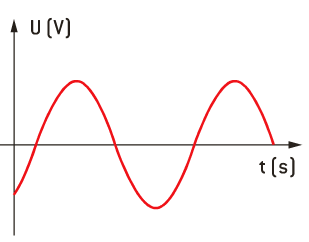
\includegraphics[scale=0.8]{bilan2}
		\end{center}
	
	Un voltmètre branché aux bornes d'un générateur permet de mesurer la tension électrique à différents instants. Un graphique est établi à partir de ces mesures pour visualiser les variations de tension. Ce graphique représente l'évolution de la tension $U$ (en $V$) en fonction du temps $t$ (en $s$).
	
	}
\end{mybilan}